\documentclass[10pt]{article}

\usepackage[utf8]{inputenc}
\usepackage[hungarian]{babel}
\usepackage[a4paper, margin=1in]{geometry}

\usepackage{listings}
\usepackage{graphicx}
\usepackage{hyperref}
\usepackage{courier}

% kód font
\lstset{basicstyle=\ttfamily}

% kódban ékezet
\lstset{literate=
  {á}{{\'a}}1 {é}{{\'e}}1
}

\hyphenation{Elasticsearch}

\title{Web scraping alapú tartalomaggregátor \\ \Large{Témalaboratórium}}
\author{Mihályi Viktor}
\date{2018. 12. 13.}

\begin{document}

\maketitle
\tableofcontents

\section{Célok}
Az alkalmazás célja aggregálni az ismert használt termékek eladására szolgáló oldalakról a számítógép alkatrészeket, majd ehhez felhasználói felületet nyújtani. Ez a dokumentum a web scraping rész megvalósítását tárgyalja.

\section{Architektúra}
\begin{center}
    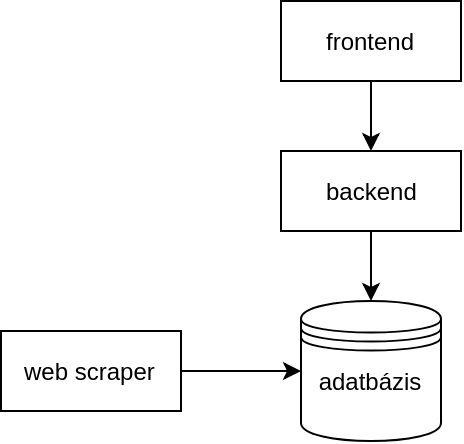
\includegraphics[scale=0.33]{arch.png}
\end{center}

A központban egy Elasticsearch adatbázis van, ami gyors keresést biztosít a rendszernek. A .NET Core alapú backend egy REST API-t kínál a frontend-nek. A frontend Vue.js framework-öt használ. A web scraping modul Python nyelven íródott, függetlenül működik a backendtől és frontendtől, csak az adatbázissal kommunikál.


\section{Web scraping modul áttekintése}
A web scraping modul feladata a weboldalak bejárása, és az azokon található adatok elmentése.

Azt, hogy az oldalakat milyen sorrendben látogatja meg, és azokon milyen adatokat ment el, a \lstinline{spiders} mappában található JSON konfigurációs fájlok írják le. Egy fájl egy oldalon lévő működést írja le. A projektünk 3 apróhírdetés oldalt jár be, ez 3 különböző konfigurációt jelent.

\subsection{Konfugirációs fájl}
Tervezésnél szempont volt, hogy könnyű legyen új oldalakat felvenni a meglevők közé, illetve rugalmas legyen az elmentett adatok listája is. Ennek érdekében az oldalak bejárását, illetve azon az adatok elmentését  JSON fájlok írják le.

Az alapötlet az volt, hogy egy scraper két dolgot csinálhat egy oldalon: elment adatokat, valamint kikeresi a következő linkeket, amikre továbbmegy. Ezért a konfigurációban metódusokat adhatunk meg, amik erre a két funkcióra képesek. A metódusokat a nevükkel azonosítjuk, így lehetőség van rekurzív metódusok írására. Ezzel a megoldással bármely oldal struktúráját bejárhatjuk. 

Mivel ezt a szöveges fájlt könnyű elgépelni, ezért az alapvető hibákat a egy validator modul ellenőrzi. Ezek a hibák a \lstinline{config_validator.py} fájl részletezésénél vannak leírva.

Egy valid konfiguráció a következőket tartalmazza:
\begin{lstlisting}[frame=single]
{
    "name": "example bot",
    "enabled": true,            // opcionális, alapértelmezetten true 
    "starting_urls": [ ... ],
    "methods": [ ... ],
    "data_collectors": [ ... ],
}
\end{lstlisting}

A \lstinline{"methods"} részben metódusokat adhatunk meg. A \lstinline{"call_collectors"} megadja, hogy melyik adatgyűjtőket futtassa, a \lstinline{"follow_links"} pedig a következő oldalra mutató linkeket. Egy metódust a következő formában kell megadni:
\begin{lstlisting}[frame=single]
{
    "method_name": "example method", 
    "follow_links": [ ... ],         // opcionális
    "call_collectors": [ ... ],      // opcionális
}
\end{lstlisting}

A \lstinline{"data_collectors"} részben az adatok begyűjtését írjuk le, minden gyűjtőnek kell adni nevet, valamit azt, hogy milyen attribútumokat fog elmenteni.
\begin{lstlisting}[frame=single]
{
    "name": "example collector",
    "properties":
    [
        {
            "name": "title",
            "selector": { ... }
        },
        {
            "name": "description",
            "selector": { ... }
        },
    ]
}
\end{lstlisting}


A \lstinline{"follow_links"} részben egy szelektor szerepel, valamint az a metódus, aminek le kell majd futnia azon az oldalon. 
\begin{lstlisting}[frame=single]
{
    "selector": { ... },
    "call_method": "example method"
},
\end{lstlisting}


Egy szelektor leírása. A típus lehet \lstinline{"css"}, \lstinline{"xpath"}, vagy\lstinline{ "regex"}. A \lstinline{"parse_as"} megadja az utófeldogozás módját, alapértelmezetten \lstinline{"raw"}, lehet még \lstinline{"text"} és \lstinline{"number"}.
\begin{lstlisting}[frame=single]
{
    "type": "css",
    "command": "#product-price", 
    "parse_as": "number"
}
\end{lstlisting}

Végül a \lstinline{"starting_urls"} alatt megadjuk, hogy honnan induljon egy scraper, majd erre milyen metódust hívjon. Ilyen objektumokat írhatunk le:
\begin{lstlisting}[frame=single]
{
    "urls": [ "https://example.com", ... ],
    "method": "example method"
}
\end{lstlisting}

A mi esetünkben így néz ki a \url{https://hardverapro.hu} scrapeléséhez szükséges \lstinline{"starting_urls"} és \lstinline{"methods"} rész. A kezdőoldalon meghívja a \lstinline{"visit_products"}-ot, ami generál kéréseket az összes termék meglátogatásához (\lstinline{"follow_links"} első objektumában), majd utána kikeresi a következő oldalra mutató linket, és azon meghívja ugyan ezt a metódust (\lstinline{"follow_links"} második objektuma). Minden termék oldalán lefut a \lstinline{"termek"} nevű gyűjtő.
\begin{lstlisting}[frame=single]
"starting_urls": [{
    "urls": ["https://hardverapro.hu/aprok/index.html"],
    "method": "visit_products"
}],
"methods": [
    {
        "method_name": "visit_products",
        "follow_links": [
            {
                "selector": {
                    "type": "css",
                    "command": "[data-uadid] > a::attr(href)"
                },
                "call_method": "collect_data"
            },
            {
                "selector": {
                    "type": "xpath",
                    "command":
                        "//*[@id=\"forum-nav-top\"]/ul[1]/li[4]/a/@href"
                },
                "call_method": "visit_products"
            }
        ]
    },
    {
        "method_name": "collect_data",
        "call_collectors": [ "termek" ]
    }
]
...
\end{lstlisting}



\section{Külső könyvtárak}

\subsection{Scrapy}
A scrapelés központi eleme, rengeteg dolgot leegyszerűsít. \cite{scrapy_glance}
A következőket kezeli:
\begin{itemize}
  \item HTTP kérések, átirányítások kezelése
  \item kérések között várakozás
  \item robots.txt betartása
  \item több scraper párhuzamos futtatása
  \item HTML dokumentum feldolgozása XPath/CSS szelektorokkal 
\end{itemize}
Egy önálló web scaper ágenst spider-nek nevez a könyvtár, a program is ezt az elnevezést fogja használni.


\subsection{Beautiful Soup (bs4)}
Mivel a Scrapy rendelkezik CSS és XPath szelektorokkal, ezért csak minimálisan volt szükség erre a könyvtárra. Ezzel viszont kényelmesebb volt a szöveg utófeldolgozása, amikor egy HTML blokkot összefüggő szöveggé kell alakítanunk.

\subsection{Python Elasticsearch Client (elasticsearch-py)}
A könyvtár biztosítja a kommunikációt az Elasticsearch adatbázisunkhoz. A \lstinline{dbmanager.py} tartalmazza azt a néhány sort, amivel dokumentumokat (relációs adatbázisokban a sor megfelelője) tudunk felvenni az adatbázisba.

\section{Forráskód}

A függőségi gráf:
\begin{center}
    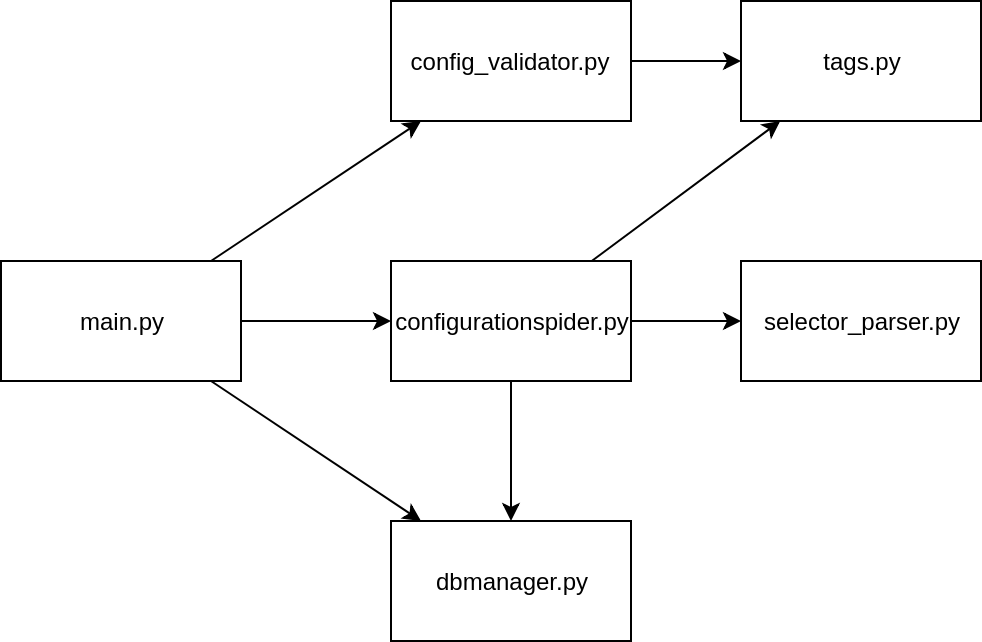
\includegraphics[scale=0.33]{scraper_arch.png}
\end{center}

\subsection{main.py}
Ez a fájl tartalmazza a main függvényt. Összeszedi a \lstinline{spiders} mappában található konfigurációkat, validálja, majd egy közös process-be rakva elindítja őket. Az ágensek csak akkor indulnak, ha van adatbázis kapcsolat.

\subsection{settings.py}
A Scrapy könyvtárhoz tartozó beállításokat tartalmazza. \cite{scrapy_settings}

Beállítunk egy 5 másodperces késleltetést a kérések között (\lstinline{DOWNLOAD_DELAY}). Ez a késleltetés csak konfigurációnként értendő, tehát a különböző weboldalakat párhuzamosan járja be. Megad egy \lstinline{User agent}-et, amit minden kérés header részébe betesz (\lstinline{USER_AGENT}).

Ez a két beállítás segít abban, hogy a bejárt weboldalak ne tiltsanak le minket, és nehezebben tudjanak megkülönböztetni egy átlagos felhasználótól. Etikai szempontból is fontos, mivel nem szeretnénk túlterhelni az számunkra érdekes weboldalakat.

Megadjuk, hogy a \lstinline{robots.txt} \cite{wikipedia_robotstxt} fájlokat "betartsa", azaz eldobja azokat a kéréseket, amelyek olyan címre mutatnak, amit a weboldal nem szeretné, ha feldolgoznánk. (\lstinline{ROBOTSTXT_OBEY})

\subsection{config\_validator.py}
Egy adott konfigurációról eldönti, hogy valid-e vagy sem, ha engedélyezve van. A következők okozzák a helytelen konfigurációt:
\begin{itemize}
    \item nincs neve (ez szükséges a \lstinline{scrapy.Spider} objektumok példányosításához)
    \item nincs kezdő webcím
    \item nincs kezdő webcímet feldolgozó metódus
    \item nincsenek metódusok megadva
    \item több ugyan olyan nevű metódus/adatgyűjtő
    \item nem létező metódusra/adatgyűjtőre utalás
    \item nem használt metódus/adatgyűjtő
\end{itemize}

\subsection{configurationspider.py}
Egy \lstinline{scrapy.Spider} osztályból leszármazott osztályt tartalmaz. Egy ilyen osztály példány egy konfigurációnak megfelelő működést hajt végre. A konstruktorban megkapja a konfigurációt, a tagfüggvényeiben ez alapján fog cselekedni.

A konstruktorban kapott konfigurációt elmenti:
\begin{lstlisting}[language=Python,frame=single]
def __init__(self, **kwargs):
    super().__init__(kwargs['config'][TAG_SPIDER_NAME], **kwargs)
    self.config = kwargs['config']
    self.db = self.config['db']
\end{lstlisting}

A Scrapy minden \lstinline{scrapy.Spider} objektumon a  \lstinline{start_requests()} függvényént hívja meg először, ebben megadhatjuk azokat a HTTP kéréseket, amivel kezdeni fogja a scrapelést. Itt kikeressük a konfigurációban megadott kezdő webcímeket.
\begin{lstlisting}[language=Python,frame=single]
for starting_url in self.config['starting_urls']:
    for url in starting_url['urls']:
        yield scrapy.Request(url, 
            callback=self.parse_with_method(starting_url['method']))
\end{lstlisting}

Ha a kérés sikeres volt, a megadott callback függvényt fogja meghívni a válasszal. 
A callback függvényt egyetlen paraméterrel, a válasz objektummal fogja meghívni, viszont azt is tudnunk kéne, hogy a választ melyik metódussal akarjuk feldolgozni.
Ezért a \lstinline{parse_with_method()} egy olyan függvény, aminek egy metódus nevet megadva, visszatér egy válasz objektumot paraméterül váró függvénnyel.

\begin{lstlisting}[language=Python,frame=single]
def parse_with_method(self, method_name):
    def parse_item(response):
        ...        
    return parse_item

\end{lstlisting}

Ebben a belső függvényben két dolog történik: végrehajtja az összes definiált adatgyűjtőt \\ (\lstinline{"data_collectors"} alapján), és generálja a következő kéréseket (\lstinline{"follow_links"} alapján).

\subsection{selector\_parser.py}
Különböző szelektorokat kiértékel, majd elvégzi az utófeldolgozást. Alapesetben egy listával tér vissza, de lehetőség van megadni, hogy egyetlen visszatérő elem legyen.

Elfogadott szelektor típusok: "xpath", "css", "regex".

Az utófelolgozás a következő módokon történhet:
\begin{itemize}
    \item "raw": nincs utófeldogozás, a kiválasztott szöveggel/HTML blokkkal tér vissza
    \item "number": szöveget számmá alakít
    \item "text": több, egymásba ágyazott HTML blokkot szöveggé alakít, miközben meghagyja a sortöréseket 
\end{itemize}
    
\subsection{dbmanager.py}
Az Elasticsearch adatbázissal tarja a kapcsolat. Biztosítja új termékek felvételét, valamit egy másik függvényt, ami addig várj, amíg nem észlel adatbázis kapcsolatot. Erre azért van szükség, mivel az Elasticsearch nem tud azonnal elindulni, pedig egyszerre indítjuk a két szolgáltatást.

\subsection{tags.py}
A konfigurációs fájlokhoz tartozó sztringeket tartalmazza.

\section{Konténerizáció}
A bonyolult telepítések elkerülése érdekében lehetőség van az adatbázist és a web scraping modult konténerrel indítani.

\subsection{Docker}
A web scraping modul tartalmaz egy \lstinline{Dockerfile}-t, Docker container építéséhez. A \lstinline{Dockerfile} a következő működést írja le: létrehoz a egy \lstinline{/app} mappát, amibe bemásolja a forráskódokat, majd telepíti a szükséges Python könyvtárakat a \lstinline{requirements.txt} fájlból. A buildelés végeredmény egy $\sim$250 MB méretű image.

\subsection{Docker Compose}
A \lstinline{docker-compose.yml} fájl 2 szolgáltatást (service) orkesztrál:
\begin{itemize}
    \item \lstinline{elasticsearch}: az Elasticsearch adatbázis
    \item \lstinline{webscraping}: az web scraping modul
\end{itemize}

\section{Futtatás}
\subsection{Docker nélkül (Ubuntu)}
A \lstinline{requirements.txt} fájl tartalmazza a futtatáshoz szükséges Python csomagokat. Ezeket egy virtális környezetbe érdemes telepíteni. 
\begin{lstlisting}  
    $ sudo apt install python3 python3-venv
    $ python3 -m venv .venv
    $ source .venv/bin/activate
    $ pip3 install -r requirements.txt
\end{lstlisting}
Szükség lesz az Elasticsearch futtatására a 9200-as porton, ezt a \lstinline{src/settings.py} fáfjlban lehet módosítani.

\subsection{Docker segítségével (platformfüggetlen)}
\begin{lstlisting}
    $ docker-compose up
\end{lstlisting}

\begin{thebibliography}{9}
    \bibitem{book}
    Ryan Mitchell, \textit{Web Scraping with Python}, 2015

    \bibitem{scrapy_glance} 
    Scrapy ismeretető, \\
    \url{https://docs.scrapy.org/en/latest/intro/overview.html#what-else}
    
    \bibitem{scrapy_settings}
    Scrapy beállítások, \\
    \url{https://doc.scrapy.org/en/latest/topics/settings.html}

    \bibitem{wikipedia_robotstxt}
    robots.txt - Wikipedia, \\
    \url{https://en.wikipedia.org/wiki/Robots_exclusion_standard}
    
   \bibitem{site_elastic}
   ElasticSearch dokumentáció, \\
   \url{https://www.elastic.co/products/elasticsearch} 
\end{thebibliography}


\end{document}
